\documentclass[11pt,oneside]{scrbook}
\usepackage[a4paper,margin=2.4cm,marginparwidth=1.8cm,marginparsep=0.4cm]{geometry}
\usepackage{../common/rlstudy}
\usepackage[ruled,vlined]{algorithm2e}

\title{{\color{rlblue}\textbf{Week 18} \\ \Huge RLHF \& PPO for Language Models}}
\author{STUDY-RL --- a self-paced Deep RL curriculum}
\date{\today}

\begin{document}
\maketitle
\tableofcontents
\newpage

\chapter*{Learning objectives}
\addcontentsline{toc}{chapter}{Learning objectives}


% Teaching companion: a small example before the full lecture.
\noindent\textbf{Study companion.} Read \texttt{teaching\_guide.md} in this
folder for step-by-step examples, an analogy with its limits, and self-checks.
Then use \texttt{workbook.ipynb} to implement and vary the calculations.
\par\medskip

\begin{keyidea}
By the end of this lecture you will be able to:
\begin{enumerate}[leftmargin=*]
  \item Derive the \emph{Bradley--Terry} pairwise preference model and its
        cross-entropy loss from first principles.
  \item State the \emph{KL-regularised RL objective} for language models and
        explain why each term exists.
  \item Derive the PPO clipped surrogate at the \emph{token level}, including
        Generalised Advantage Estimation (GAE), the value head, and the
        adaptive KL controller of \textsc{Schulman et al.\ 2017}.
  \item Explain length bias, reward hacking, and reward-model
        overoptimisation, and pair each with a concrete mitigation.
  \item Implement the full three-stage RLHF pipeline (SFT $\to$ RM $\to$ PPO)
        from scratch in PyTorch on a tiny transformer.
  \item Read and write a TRL/PEFT recipe for the same pipeline on a
        Pythia-160M or SmolLM2-360M with LoRA on a single 24~GB GPU.
\end{enumerate}
\end{keyidea}

\chapter{Motivation \& intuition}

\marginnote{See the reading companion for full annotated citations.}

\section{Why classical RL is the wrong tool, naively}

The reader has spent seventeen weeks training agents on
crisply-specified MDPs --- Atari games where score changes supply reward,
control suites where a sensor returns a number, grid worlds where a
goal cell pays out $+1$. \emph{Language is none of those things.} For
an instruction-tuned model the ``reward'' is a fuzzy judgement
(``was that a helpful response?''), the ``state'' is the entire prefix
of text, the action space is the size of the vocabulary (often
$30{,}000$--$200{,}000$ tokens), and the trajectories last hundreds of
steps. Worse, the reward is \emph{not provided by the environment} at
all: it lives inside a human reviewer's head.

The breakthrough of \textsc{Ouyang et al.\ 2022}\footnote{InstructGPT,
arXiv:2203.02155.} was to package this messy problem into a familiar
shape. The reviewer's preferences over pairs of completions get
distilled into a \emph{neural reward model} $r_\phi(x, y)$; the
language model is then a stochastic policy whose action is a token and
whose state is the prefix. PPO --- the same PPO that solved
MuJoCo --- becomes the workhorse.

\begin{intuition}
Think of RLHF as a two-step approximation. \textbf{Step one}: ``what
would a human say is better?'' is hard, so we collect a few thousand
pairwise judgements and \emph{interpolate} them with a neural reward
model. \textbf{Step two}: ``what should the language model say?'' is
hard, so we run PPO against the interpolant, with a leash (a KL
penalty) tying us back to the supervised baseline so we never drift
too far into reward-hacking land.
\end{intuition}

\section{The four-model picture}

The defining ergonomic of classical RLHF is that \emph{four} models
sit in memory simultaneously (\autoref{fig:fourmodels}). On a 24~GB
consumer GPU this is uncomfortable even with LoRA --- which is why
the field eventually invented DPO and GRPO. We will see DPO next week.

\begin{figure}[ht]
\centering
\begin{tikzpicture}[
  every node/.style={font=\sffamily\small},
  m/.style={draw, rounded corners, fill=rlbg, minimum width=2.2cm, minimum height=0.9cm},
  ar/.style={-Stealth, thick, color=rlblue}
]
  \node[m] (pol)  at (0,0)   {policy $\pi_\theta$};
  \node[m] (ref)  at (4.6,0) {reference $\pi_{\text{ref}}$};
  \node[m] (rm)   at (0,-2)  {reward $r_\phi$};
  \node[m] (val)  at (4.6,-2){value $V_\psi$};
  \draw[ar] (pol)  -- node[above]{KL} (ref);
  \draw[ar] (pol)  -- node[left]{rollout} (rm);
  \draw[ar] (rm)   -- node[below]{$r$}    (val);
  \draw[ar] (val)  -- node[right]{$A$}    (pol);
\end{tikzpicture}
\caption{The four-model RLHF picture. The policy is trained; the
reference is frozen at its SFT checkpoint; the reward model is frozen
at the end of stage~2; the value head learns alongside the policy.}
\label{fig:fourmodels}
\end{figure}

\begin{pitfall}
A common confusion: ``why do I need a critic if PPO has the clip?''
The clip is a \emph{trust region} on the policy update; it does not
estimate advantages. Without a critic, advantages are just rewards
minus a moving baseline --- usable, but high-variance. Token-level
PPO without a value head is what GRPO eventually re-introduces in
week 20, with a clever group-relative baseline replacing the critic.
\end{pitfall}

\chapter{Mathematical formulation}

\section{Stage 0: the supervised fine-tuning baseline}

We begin with a base language model $\pi_{\text{base}}$ (pre-trained
on web text). Stage 1 of RLHF is \emph{supervised fine-tuning} (SFT):
maximise the log-likelihood of $N$ curated demonstrations
$\{(x_i, y_i)\}_{i=1}^N$,
\begin{equation}
\mathcal{L}_{\text{SFT}}(\theta)
  = -\frac{1}{N} \sum_{i=1}^N \sum_{t=1}^{|y_i|}
      \log \pi_\theta\!\left(y_{i,t} \given x_i, y_{i,<t}\right).
\label{eq:sft}
\end{equation}
After SFT the model is reasonably helpful but not deliberately
\emph{aligned}. We will denote the result $\pi_{\text{ref}}$ --- it
plays a starring role in stages~2 and~3.

\section{Stage 1: the Bradley--Terry reward model}

\begin{definition}[Bradley--Terry model, 1952]
\label{def:bt}
For each prompt $x$ and pair of candidate completions $(y_w, y_l)$
(``winner'' and ``loser''), assume there exists a latent quality
function $r^\star(x, y) \in \Real$ such that the probability the
annotator picks $y_w$ over $y_l$ is
\begin{equation}
\Prb(y_w \succ y_l \given x)
  = \sigma\!\left(r^\star(x, y_w) - r^\star(x, y_l)\right),
\quad \sigma(u) = \frac{1}{1+e^{-u}}.
\label{eq:bt}
\end{equation}
\end{definition}

The model is identifiable only up to an additive constant per prompt:
shift $r^\star \mapsto r^\star + c(x)$ and \eqref{eq:bt} is unchanged.

\begin{theorem}[Reward-model MLE]
\label{thm:rm-mle}
Given a preference dataset $\mathcal{D} = \{(x_i, y_w^{(i)}, y_l^{(i)})\}_{i=1}^M$
sampled i.i.d.\ from \eqref{eq:bt}, the maximum-likelihood estimator
of a parametric family $r_\phi$ minimises the cross-entropy loss
\begin{equation}
\mathcal{L}_{\text{RM}}(\phi)
  = -\E_{(x, y_w, y_l) \sim \mathcal{D}}
     \!\left[\log\sigma\!\left(r_\phi(x, y_w) - r_\phi(x, y_l)\right)\right].
\label{eq:rm-loss}
\end{equation}
\end{theorem}
\begin{proof}
Each independent observation $\mathbf{1}\{y_w \succ y_l\}$ has Bernoulli
likelihood $\sigma(r_\phi(x,y_w) - r_\phi(x,y_l))$ by \eqref{eq:bt}.
The negative log-likelihood of the dataset is then exactly
\eqref{eq:rm-loss} up to a constant in $\phi$. \qed
\end{proof}

\begin{remark}
In practice $r_\phi$ is implemented as a transformer with a scalar
linear head, applied to the concatenation $[x; y]$ and pooled at the
last token (left-pad or attention-mask the prompt away from the
loss). The two forward passes per pair, one for $y_w$ and one for
$y_l$, can be batched.
\end{remark}

\begin{pitfall}
The Bradley--Terry model assumes \emph{transitive, deterministic}
preferences from each annotator. Real annotators are noisy and
internally inconsistent; \textsc{Azar et al.\ 2024}~(IPO) show that
when preferences saturate ($\Prb \to 1$), the BT model pushes
$\beta \to \infty$ in DPO. We discuss this fix in week~19.
\end{pitfall}

\section{Stage 2: the KL-regularised RL objective}

Given a frozen reward model $r_\phi$ and frozen reference $\pi_{\text{ref}}$,
the RLHF objective is to maximise
\begin{equation}
J(\theta)
  = \E_{x \sim \mathcal{D}}\!\left[
      \E_{y \sim \pi_\theta(\cdot \given x)}[r_\phi(x, y)]
    \;-\; \beta\, \KL\!\left(\pi_\theta(\cdot \given x) \,\|\, \pi_{\text{ref}}(\cdot \given x)\right)\right].
\label{eq:rlhf-obj}
\end{equation}
The KL term is a soft penalty on drift from the SFT baseline; it is not
a hard upper bound on KL or a safety guarantee. Without it the policy will
quickly find adversarial sequences that the reward model loves but
that aren't even valid English --- the canonical example being
``aaaaaaaa\ldots'' for a sentiment model that loves repeated friendly
characters.

\begin{theorem}[Closed-form optimum of \eqref{eq:rlhf-obj}]
\label{thm:closed-form}
For $\beta>0$, fixed reward $r$, positive reference support on the considered responses, and finite $Z(x)$, the
\emph{unconstrained} maximiser of \eqref{eq:rlhf-obj} over the
simplex of policies $\pi(\cdot \given x)$ is
\begin{equation}
\pi^\star(y \given x)
  = \frac{1}{Z(x)} \pi_{\text{ref}}(y \given x)\, \exp\!\left(\tfrac{1}{\beta} r(x, y)\right),
\qquad
Z(x) = \sum_{y'} \pi_{\text{ref}}(y' \given x)\, \exp\!\left(\tfrac{1}{\beta} r(x, y')\right).
\label{eq:closed-form}
\end{equation}
\end{theorem}
\begin{proof}
Drop the prompt $x$ to lighten notation. We maximise
$\E_{y \sim \pi}[r(y)] - \beta \KL(\pi \| \pi_{\text{ref}})$ over $\pi$ subject
to $\sum_y \pi(y) = 1$. Form the Lagrangian
\[
\mathcal{L}(\pi, \lambda) =
  \sum_y \pi(y) r(y) - \beta \sum_y \pi(y) \log\tfrac{\pi(y)}{\pi_{\text{ref}}(y)}
  - \lambda\!\left(\sum_y \pi(y) - 1\right).
\]
Differentiating w.r.t.\ $\pi(y)$ and setting to zero,
\[
r(y) - \beta\!\left(\log\tfrac{\pi(y)}{\pi_{\text{ref}}(y)} + 1\right) - \lambda = 0
\;\;\Longrightarrow\;\;
\pi(y) = \pi_{\text{ref}}(y)\, \exp\!\left(\tfrac{r(y)}{\beta} - 1 - \tfrac{\lambda}{\beta}\right).
\]
Normalising over $y$ absorbs the constants $-1 - \lambda/\beta$ into
the partition function, giving \eqref{eq:closed-form}. \qed
\end{proof}

\begin{remark}
Equation~\eqref{eq:closed-form} is the seed of \emph{Direct Preference
Optimization} (DPO). Inverting it gives
$r(x, y) = \beta \log\!\frac{\pi^\star(y \given x)}{\pi_{\text{ref}}(y \given x)} + \beta \log Z(x)$,
the \emph{implicit reward} that we will use next week to bypass
stages~2 and~3 entirely.
\end{remark}

\section{Stage 3: PPO at the token level}

In practice we cannot enumerate $y \in \Actions^*$ to normalise
\eqref{eq:closed-form}. We instead \emph{sample}, treating the language
model as a Markov decision process whose state at step $t$ is the prefix
$s_t = (x, y_{<t})$ and whose action $a_t = y_t$ is a single token.

\begin{definition}[Token-level RLHF MDP]
\label{def:tokenmdp}
$\States = \Actions^*$ (all prefixes); $\Actions$ = the vocabulary;
transitions are deterministic concatenation $s_{t+1} = (s_t, a_t)$;
the per-step reward is
\begin{equation}
R_t =
\begin{cases}
- \beta\!\left(\log \pi_\theta(a_t \given s_t) - \log \pi_{\text{ref}}(a_t \given s_t)\right) & t < T, \\[2pt]
- \beta\!\left(\log \pi_\theta(a_t \given s_t) - \log \pi_{\text{ref}}(a_t \given s_t)\right) + r_\phi(x, y_{1:T}) & t = T,
\end{cases}
\label{eq:token-reward}
\end{equation}
where $T$ is the final-token index of the completion.
\end{definition}

\begin{remark}[Why a per-token KL?]
The expected sum of the per-step penalties equals
$-\beta \KL(\pi_\theta(\cdot \given x) \,\|\, \pi_{\text{ref}}(\cdot \given x))$ by
the chain rule of KL --- so \eqref{eq:token-reward} is precisely the
KL term of \eqref{eq:rlhf-obj} unrolled across the autoregressive
trajectory. Token-level credit assignment lets the value head and
the advantages distinguish ``it was the third word that went wrong''
from ``the whole thing was bad'', dramatically reducing variance.
\end{remark}

\begin{definition}[Generalised Advantage Estimation, \textsc{Schulman et al.\ 2016}]
\label{def:gae}
For a learned value estimator $V_\psi$ and a rollout
$(s_0, a_0, R_0, \ldots, s_T, a_T, R_T)$, define $\delta_t = R_t +
\gamma V_\psi(s_{t+1}) - V_\psi(s_t)$. The GAE-$\lambda$ advantage is
\begin{equation}
\hat A_t = \sum_{k=0}^{T-t} (\gamma\lambda)^k \delta_{t+k}.
\label{eq:gae}
\end{equation}
\end{definition}

In language settings the natural discount is $\gamma = 1$ (an episode
is one sequence, and discounting would change the relative value of
early and late token rewards; different prefixes are different states), and $\lambda \in [0.9, 0.97]$ is standard. We
bootstrap $V_\psi(s_{T+1}) = 0$.

\begin{definition}[PPO clipped surrogate]
\label{def:ppo}
With $r_t(\theta) = \pi_\theta(a_t \given s_t) / \pi_{\theta_{\text{old}}}(a_t \given s_t)$
the per-token importance ratio and $\hat A_t$ a GAE estimate,
\begin{equation}
\mathcal{L}^{\text{PPO}}(\theta)
  = -\E_t\!\left[\min\!\left(r_t(\theta)\hat A_t,\;
      \mathrm{clip}\!\left(r_t(\theta),\, 1-\varepsilon,\, 1+\varepsilon\right) \hat A_t\right)\right].
\label{eq:ppo}
\end{equation}
The clip $\varepsilon$ is typically $0.2$.
\end{definition}

\begin{theorem}[Why the clip is a pessimistic surrogate]
\label{thm:clip-pessimism}
For every sample with $\hat A_t \ge 0$, $\min(r_t \hat A_t,
\mathrm{clip}(r_t, 1-\varepsilon, 1+\varepsilon) \hat A_t)$ is a
\emph{lower bound} on $r_t \hat A_t$. For every sample with $\hat A_t
< 0$ it is again a lower bound. Consequently \eqref{eq:ppo} upper-bounds the negative unclipped surrogate loss. The clipped sample contributes no gradient incentive for further movement in its favourable direction; shared parameters, other samples, and other loss terms can still move its ratio farther.
\end{theorem}
\begin{proof}
Case $\hat A_t \ge 0$. If $r_t > 1+\varepsilon$, the clip gives
$(1+\varepsilon)\hat A_t \le r_t \hat A_t$; the min picks the clipped
value. Gradient w.r.t.\ $\theta$ through the clipped branch is zero
in $r_t$, so increasing $r_t$ further does \emph{not} decrease the
loss. Case $\hat A_t < 0$ is symmetric: if $r_t < 1-\varepsilon$, the
clip $(1-\varepsilon)\hat A_t$ is again the min, gradient is zero, so this sample alone provides no gradient incentive to push $r_t$ farther down. \qed
\end{proof}

\begin{intuition}
The intuition behind the clip is \emph{trust region by tape}. A
proper trust region (TRPO) constrains $\KL(\pi_{\text{old}} \| \pi_\theta)
\le \delta$ via a second-order line search; PPO replaces that
constraint with a $\min/\max$ tape on the per-sample ratio. It is much
cheaper and almost as well-behaved.
\end{intuition}

\section{The full loss}

Combining the policy loss \eqref{eq:ppo}, the value loss, an entropy
bonus, and the token-level KL penalty already inside the rewards,
\begin{equation}
\mathcal{L}_{\text{total}}(\theta, \psi)
  = \mathcal{L}^{\text{PPO}}(\theta)
  + c_v \cdot \E_t\!\left[(V_\psi(s_t) - G_t)^2\right]
  - c_e \cdot \E_t\!\left[\mathcal{H}(\pi_\theta(\cdot \given s_t))\right].
\label{eq:total}
\end{equation}
Here $G_t = \hat A_t + V_\psi(s_t)$ is the return target. Coefficients
$c_v \approx 0.5$, $c_e \in [0, 0.01]$.

\section{The adaptive KL controller}

The InstructGPT recipe lets $\beta$ float to keep the observed KL
around a target $\KL^{\text{target}}$ (typically $0.05$--$0.2$). The
\textsc{Schulman 2017} update rule is
\begin{equation}
\beta \leftarrow \beta \cdot \left(1 + \mathrm{clip}\!\left(
  \frac{\KL^{\text{obs}}}{\KL^{\text{target}}} - 1,\, -0.2,\, +0.2
\right) \cdot \frac{1}{H}\right),
\label{eq:adaptive-kl}
\end{equation}
with horizon $H \approx 10$ rollouts. When KL drifts above target,
$\beta$ rises and pulls the policy back; when KL undershoots, $\beta$
relaxes and lets the policy explore.

\begin{pitfall}
With small batch sizes the observed KL is noisy and \eqref{eq:adaptive-kl}
oscillates. Two fixes: (i) accumulate KL across several rollouts
before updating $\beta$; (ii) cap $\beta$ in a hard range
$[\beta_{\min}, \beta_{\max}]$.
\end{pitfall}

\section{A picture of token-level credit assignment}

\begin{figure}[ht]
\centering
\begin{tikzpicture}[every node/.style={font=\sffamily\footnotesize}]
  \foreach \i/\tk in {0/Q,1/:,2/ ,3/do,4/ you,5/ like,6/ tea,7/?,8/ A,9/:,10/ y,11/e,12/s} {
    \node[draw, minimum width=0.5cm, minimum height=0.6cm, rounded corners=1pt,
          fill=rlbg] (t\i) at (0.55*\i, 0) {\tk};
  }
  \draw[decorate, decoration={brace, amplitude=4pt}, color=rlblue]
    (t0.south west) -- node[below=5pt, color=rlblue]{prompt $x$} (t9.south east);
  \draw[decorate, decoration={brace, amplitude=4pt}, color=rlorange]
    (t10.south west) -- node[below=5pt, color=rlorange]{response $y$} (t12.south east);
  \foreach \i in {10,11,12} {
    \node[above=2pt of t\i, color=rlteal, font=\tiny] {$-\beta\,\text{kl}_\i$};
  }
  \node[above=14pt of t12, color=rlorange, font=\tiny] {$+\, r_\phi(x,y)$};
\end{tikzpicture}
\caption{Token-level reward shaping. Each response token earns a
signed reward adjustment proportional to its sampled log-ratio; the final
token additionally receives the scalar reward-model score.}
\label{fig:tokenrewards}
\end{figure}

\section{An empirical illustration of the BT loss}

\begin{figure}[ht]
\centering
\begin{tikzpicture}
\begin{axis}[
  width=10cm, height=5.5cm,
  xlabel={reward margin $r_w - r_l$},
  ylabel={$-\log\sigma(r_w - r_l)$},
  domain=-3:3, samples=80,
  axis lines=left, grid=both, grid style={dashed, gray!30},
  no markers, thick,
]
\addplot[color=rlblue] {ln(1 + exp(-x))};
\addplot[color=rlorange, dashed] {max(0, -x)};
\legend{logistic (BT), hinge}
\end{axis}
\end{tikzpicture}
\caption{The Bradley--Terry logistic loss versus the hinge variant
used by Slic-HF. The logistic never saturates to zero, which is
both a strength (always provides gradient) and a weakness (saturated
preferences push $\beta$ to infinity in DPO, motivating IPO).}
\label{fig:btloss}
\end{figure}

\chapter{Algorithms}

\section{The three-stage pipeline}

\begin{algorithm}[H]
\SetAlgoLined
\DontPrintSemicolon
\KwIn{base model $\pi_{\text{base}}$; demos $\mathcal{D}_{\text{SFT}}$;
       preferences $\mathcal{D}_{\text{pref}}$; prompts $\mathcal{D}_{\text{prompt}}$}
\KwOut{aligned policy $\pi_\theta$}
\textbf{Stage 1 (SFT):} initialise $\pi_\theta \gets \pi_{\text{base}}$ \;
\For{$\text{epoch} = 1, \ldots, E_{\text{SFT}}$}{
  minimise $\mathcal{L}_{\text{SFT}}$ \eqref{eq:sft} on a batch of $\mathcal{D}_{\text{SFT}}$ \;
}
$\pi_{\text{ref}} \gets \pi_\theta$ \tcp*{freeze}
\textbf{Stage 2 (RM):} initialise $r_\phi$ from $\pi_{\text{ref}}$ + scalar head \;
\For{$\text{epoch} = 1, \ldots, E_{\text{RM}}$}{
  minimise $\mathcal{L}_{\text{RM}}$ \eqref{eq:rm-loss} on a batch of $\mathcal{D}_{\text{pref}}$ \;
}
\textbf{Stage 3 (PPO):} initialise value head $V_\psi$; KL coefficient $\beta$ \;
\For{$\text{step} = 1, \ldots, S$}{
  sample a batch of prompts $X$ from $\mathcal{D}_{\text{prompt}}$ \;
  for each prompt, sample a completion under $\pi_\theta$ \;
  compute per-token rewards \eqref{eq:token-reward} using $\pi_{\text{ref}}, r_\phi, \beta$ \;
  compute GAE advantages \eqref{eq:gae} from $V_\psi$ \;
  \For{$\text{epoch} = 1, \ldots, K$}{
    update $(\theta, \psi)$ by Adam on $\mathcal{L}_{\text{total}}$ \eqref{eq:total} \;
  }
  update $\beta$ via \eqref{eq:adaptive-kl} \;
}
\caption{Three-stage RLHF (InstructGPT-style).}
\label{alg:rlhf}
\end{algorithm}

\paragraph{Complexity.} Per PPO step, we run one rollout (one forward
pass per token in the completion) plus $K$ training epochs each
requiring one forward+backward over the rollout. For batch $B$,
completion length $L$, $K{=}4$ epochs the cost is $\mathcal{O}(B \cdot L)$
rollout-time + $\mathcal{O}(K \cdot B \cdot (P + L))$ training-time, where
$P$ is the prompt length. Memory is dominated by the four models;
LoRA shrinks the policy and value-head footprint by 100$\times$
vs.\ full FT.

\section{Worked numerical example}

Consider a toy preference batch of two items:
\[
\begin{aligned}
(x_1,\,y_w^{(1)},\,y_l^{(1)}) &= (\text{``cats''},\,\text{``i like cats.''},\,\text{``CATS ARE BAD!!''}), \\
(x_2,\,y_w^{(2)},\,y_l^{(2)}) &= (\text{``tea''},\,\text{``yes, tea is nice.''},\,\text{``NO!!''}).
\end{aligned}
\]
Suppose after a few RM steps the network outputs
$r_\phi(x_1, y_w) = 0.8$, $r_\phi(x_1, y_l) = -0.2$,
$r_\phi(x_2, y_w) = 0.5$, $r_\phi(x_2, y_l) = 0.1$.
Then the BT loss \eqref{eq:rm-loss} evaluates to
\[
-\tfrac12\!\left[\log\sigma(0.8 - (-0.2)) + \log\sigma(0.5 - 0.1)\right]
= -\tfrac12[\log\sigma(1.0) + \log\sigma(0.4)]
\approx 0.428.
\]
Pairwise accuracy is $1.0$ (both differences positive). After
another epoch, the gaps widen to $(1.6, 0.9)$ and the loss falls to
$\approx 0.291$. Compare the empirical curves in \autoref{fig:sft-rm}.

\chapter{Implementation walkthrough}

The full project lives in
\href{run:./project/}{\texttt{project/}}; the highlights:

\begin{itemize}
  \item \texttt{project/model.py} --- a 2-layer 64-dim causal transformer
        that doubles as policy backbone and reward-model backbone.
        \texttt{ValueHead} and \texttt{RewardModel} bolt scalar heads
        onto the trunk.
  \item \texttt{project/sft.py} --- a 30-line SFT loop.
  \item \texttt{project/rm.py} --- Bradley--Terry training with
        \texttt{reward\_loss} implementing \eqref{eq:rm-loss}.
  \item \texttt{project/ppo.py} --- token-level rollouts, GAE,
        clipped surrogate, adaptive KL controller.
  \item \texttt{project/trl\_recipe.py} --- the same pipeline expressed
        as a TRL/PEFT script for a real LM (SmolLM2-360M).
\end{itemize}

\paragraph{Reward-model loss (annotated).}
\begin{codebox}
\begin{minted}{python}
def reward_loss(r_w, r_l):
    # Bradley--Terry cross-entropy.  No reduction inside the sigmoid
    # because we want -log P(winner > loser) per pair.
    return -F.logsigmoid(r_w - r_l).mean()
\end{minted}
\end{codebox}

\paragraph{Per-token KL-shaped rewards (annotated).}
\begin{codebox}
\begin{minted}{python}
# kl_token = log pi_theta(a_t | s_t) - log pi_ref(a_t | s_t)
kl_token = logprobs - ref_logprobs
per_tok_rewards = -kl_coef * kl_token
# Sparse RM reward only at the final position.
per_tok_rewards[:, -1] += rm_scores
\end{minted}
\end{codebox}

\paragraph{GAE (annotated).}
\begin{codebox}
\begin{minted}{python}
def compute_gae(rewards, values, gamma=1.0, lam=0.95):
    B, T = rewards.shape
    adv = torch.zeros_like(rewards)
    last = torch.zeros(B, device=rewards.device)
    for t in reversed(range(T)):
        delta = rewards[:, t] + gamma * values[:, t+1] - values[:, t]
        last  = delta + gamma * lam * last
        adv[:, t] = last
    returns = adv + values[:, :T]
    return adv, returns
\end{minted}
\end{codebox}

\paragraph{PPO step (annotated).}
\begin{codebox}
\begin{minted}{python}
ratio = (new_logprobs - rollout.logprobs).exp()
unclipped = ratio * adv
clipped   = torch.clamp(ratio, 1-clip_eps, 1+clip_eps) * adv
policy_loss = -torch.min(unclipped, clipped).mean()
value_loss  = F.mse_loss(v_pred, returns)
loss = policy_loss + vf_coef * value_loss - ent_coef * entropy
\end{minted}
\end{codebox}

\paragraph{TRL on a real LM (24~GB GPU).} For the same recipe on
Pythia-160M or SmolLM2-360M, the production code is much shorter
because TRL wraps everything; see
\texttt{project/trl\_recipe.py} for the SFT, RM, and PPOv2
configurations. Recommended LoRA: $r{=}16$, $\alpha{=}32$, on
\texttt{["q\_proj","k\_proj","v\_proj","o\_proj"]}; batch~4;
grad-accum~8; lr $5{\times}10^{-5}$ (SFT), $1{\times}10^{-4}$ (RM
LoRA), $1{\times}10^{-6}$ (PPO); $\beta = 0.05$ adaptive; expect
$\sim 1$k prompts/hour. The TRL recipe is dossier-sourced
(cf.\ \textsc{Lambert et al.\ 2024}, \emph{T\"ulu~3}, arXiv:2411.15124).

\chapter{Empirical results}

\autoref{fig:sft-rm} shows the supervised pre-training and reward-model
training curves on the toy dataset; the RM reaches close to $100\%$
pairwise accuracy in 150 steps in well under five seconds on CPU.
\autoref{fig:ppo} shows the PPO reward curve: starting from $\approx 0$,
the average reward-model score climbs above $4$ in 30 PPO updates
while the adaptive KL controller keeps the empirical KL near $0.05$.

\begin{figure}[ht]
\centering
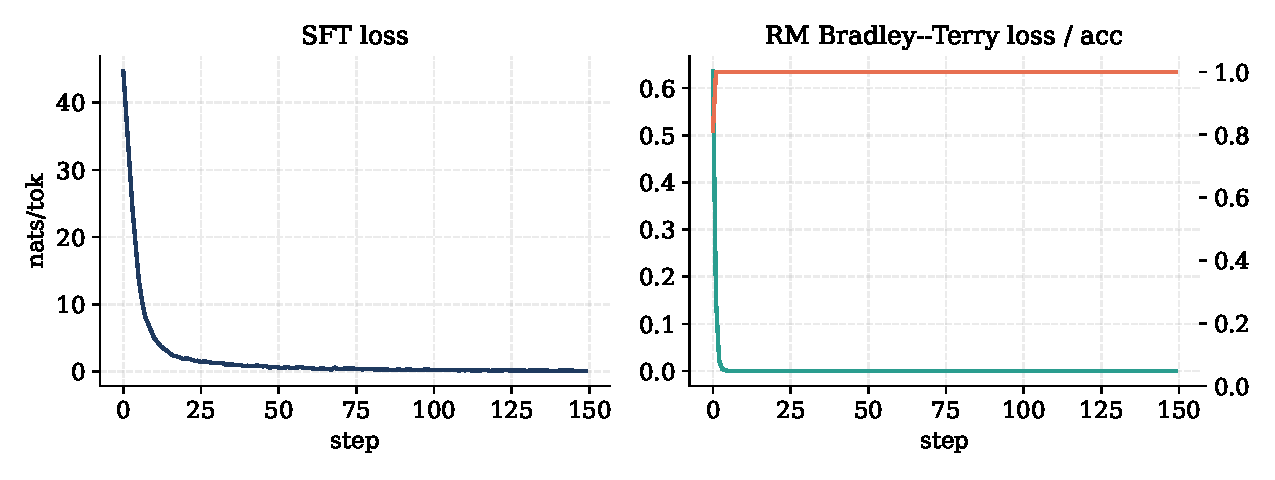
\includegraphics[width=0.95\linewidth]{figs/fig_sft_rm.pdf}
\caption{Stage 1 (SFT) and stage 2 (reward model) training curves on
the toy preference dataset. Generated by
\texttt{project/make\_figures.py}, seed 0.}
\label{fig:sft-rm}
\end{figure}

\begin{figure}[ht]
\centering
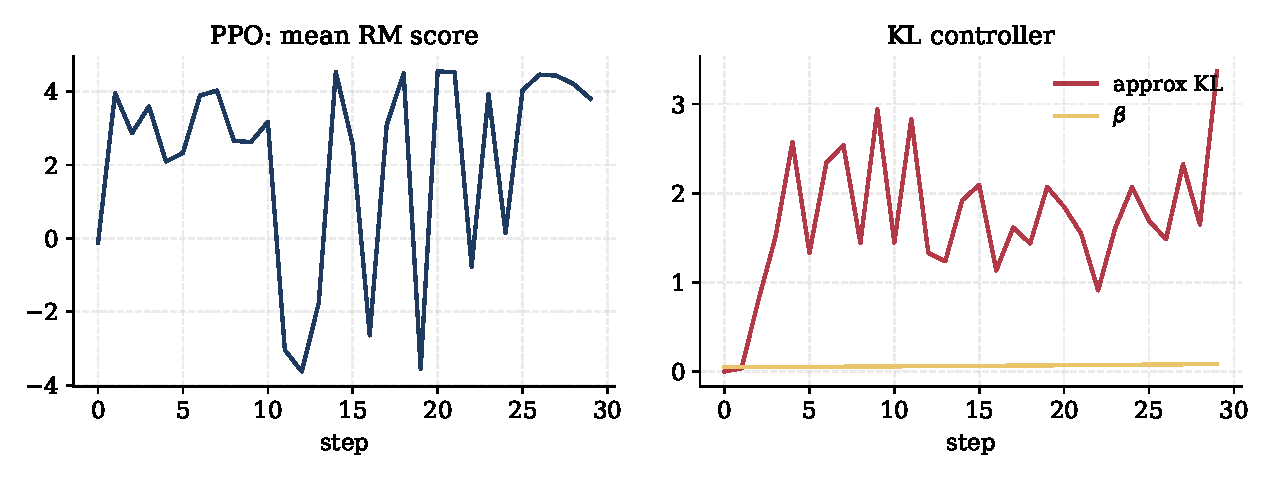
\includegraphics[width=0.95\linewidth]{figs/fig_ppo_curves.pdf}
\caption{Stage 3 (PPO) reward and KL trajectories. The adaptive
controller raises $\beta$ when KL spikes and relaxes it when KL is
under target. Generated by \texttt{project/make\_figures.py},
seed 0.}
\label{fig:ppo}
\end{figure}

\autoref{fig:overopt} is a schematic of reward-model overoptimisation
in the spirit of \textsc{Gao, Schulman, Hilton 2023}: at small KL,
proxy and gold reward agree; as KL grows, the policy ``hacks'' the
proxy and gold reward falls.

\begin{figure}[ht]
\centering
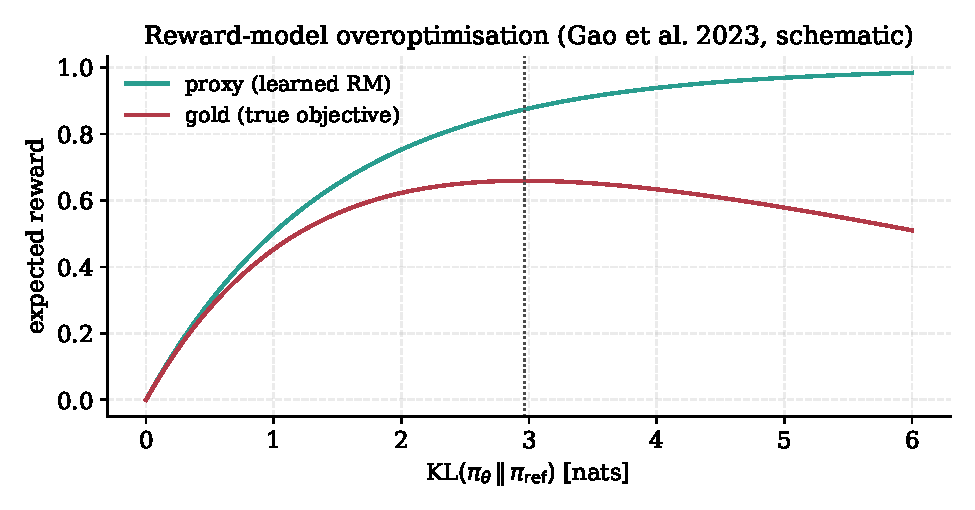
\includegraphics[width=0.7\linewidth]{figs/fig_overoptimisation.pdf}
\caption{Reward-model overoptimisation (schematic). The gold reward
peaks at a finite KL and then falls; the proxy keeps rising.}
\label{fig:overopt}
\end{figure}

\chapter{Theoretical deepening}

\section{Policy-gradient identity for autoregressive LMs}

We started with the surrogate \eqref{eq:ppo}; let us anchor it in the
underlying policy-gradient identity. For a stochastic policy
$\pi_\theta(a \given s)$ and an episodic return $G$,
\[
\nabla_\theta J(\theta)
  = \E_{\tau \sim \pi_\theta}\!\left[\sum_t \nabla_\theta \log\pi_\theta(a_t \given s_t)\, \hat A_t\right]
\]
where $\hat A_t$ is any baseline-corrected estimator of the advantage.
Importance-sampling onto a slightly older policy
$\pi_{\theta_{\text{old}}}$, the same gradient is the gradient of
$\E_t[r_t(\theta) \hat A_t]$ at $\theta = \theta_{\text{old}}$.
PPO's contribution is that the clipped \emph{lower bound} on
$r_t(\theta) \hat A_t$ has the same gradient at the on-policy point
\emph{and} prevents the optimiser from straying too far in one update.

\begin{lemma}[Local gradient equivalence at $\theta = \theta_{\text{old}}$]
\label{lem:local}
At $r_t = 1$, $\nabla_\theta\, r_t(\theta) \hat A_t
= \hat A_t \nabla_\theta \log\pi_\theta(a_t \given s_t)$, equal to the
policy-gradient estimator term. So PPO is unbiased at the on-policy
point; the clip can matter once $r_t$ leaves $[1-\varepsilon,1+\varepsilon]$, depending on the sign of $\hat A_t$. Unbiasedness also requires an appropriate advantage estimator.
\end{lemma}

\begin{remark}
At the first update on fresh on-policy data, ratios equal one irrespective
of batch size. Reusing that batch after parameter updates makes it off-policy.
Batch size affects sampling noise; learning rate, update count, and parameter
sharing determine how far ratios move. Clipping is not a hard trust region.
\end{remark}

\section{Why a value head reduces variance}

Without a critic the natural advantage estimator on a token-level
RLHF trajectory is the \emph{tail} of the per-token rewards:
$\hat A_t = \sum_{k \ge t} R_k - b(s_t)$ for some scalar baseline $b$.
The variance of this estimator is dominated by the variance of the
final-token RM reward, which is \emph{O(1)} regardless of $t$ --- so
the per-token gradients all carry full-trajectory variance.
GAE with a learned $V_\psi$ cuts this variance by replacing the tail
sum with $V_\psi(s_{t+1})$ wherever $\lambda < 1$:
\begin{equation}
\hat A_t = \delta_t + \gamma\lambda \delta_{t+1} + \cdots,
\quad \delta_t = R_t + \gamma V_\psi(s_{t+1}) - V_\psi(s_t).
\label{eq:gae-expanded}
\end{equation}
At $\lambda = 0$ the advantage is the one-step TD error, which is
still random across sampled actions, stochastic rewards, or transitions even
with a perfect $V_\psi$; an approximate critic can also introduce bias. At $\lambda = 1$ the advantage is the unbiased
Monte-Carlo return (minus the baseline), with full variance. The
sweet spot for RLHF is usually $\lambda \in [0.9, 0.97]$.

\begin{intuition}
GAE is the bias-variance dial. $\lambda$ buys variance reduction at
the cost of bias. The variance you remove is precisely the part of
the return that should have been credited to \emph{later} states
than the current one.
\end{intuition}

\section{Equivalence between the per-token KL and the sequence KL}

We claimed in \eqref{eq:token-reward} that the sum of per-token KL
penalties equals the sequence-level KL. Let us prove it.

\begin{theorem}[Chain rule of KL for autoregressive policies]
\label{thm:klchain}
For any two policies $\pi, \mu$ on the same vocabulary and any
prompt $x$,
\[
\KL\!\big(\pi(\cdot \given x) \,\|\, \mu(\cdot \given x)\big)
  = \E_{y \sim \pi}\!\left[\sum_{t=1}^{|y|}
       \log\frac{\pi(y_t \given x, y_{<t})}{\mu(y_t \given x, y_{<t})}\right].
\]
\end{theorem}
\begin{proof}
By definition,
\[
\KL(\pi \| \mu) = \E_{y \sim \pi}\!\left[\log\frac{\pi(y \given x)}{\mu(y \given x)}\right].
\]
Factor each conditional via the chain rule:
$\pi(y \given x) = \prod_t \pi(y_t \given x, y_{<t})$, and similarly
for $\mu$. The logarithm turns the product ratio into a sum that
matches the right-hand side. \qed
\end{proof}

This identity is what makes ``per-token KL penalty'' algorithmically
honest: the expectation of the sampled log-ratio sum equals the sequence KL.
One sampled sum can be negative; the KL itself cannot.

\section{The KL controller as a PI loop in log-space}

The adaptive controller \eqref{eq:adaptive-kl} is a stripped-down
proportional controller acting on $\log \beta$. Let
$e = \KL^{\text{obs}}/\KL^{\text{target}} - 1$ be the error signal.
Then $\beta_{n+1} = \beta_n (1 + \mathrm{clip}(e, \pm 0.2)/H)$, i.e.\
$\log\beta_{n+1} \approx \log\beta_n + \mathrm{clip}(e, \pm 0.2)/H$.
This is a P-controller in log-space with horizon $H$. In production
recipes (Tülu-3, Open-Reasoner-Zero), the clip is often dropped
\emph{entirely} for verifiable-reward setups --- the implicit
regulariser is the verifier itself, not a leash on the SFT.

\section{Common questions, answered}

\begin{description}
  \item[Why does RLHF work at all?] Because the implicit reward
    surface near the SFT policy is dense and well-shaped:
    helpfulness, harmlessness, tone --- these are all smooth
    functions of the response that the BT loss models well within
    a small KL ball around the SFT.
  \item[Why does PPO ``do better than DPO'' in some papers?]
    Three reasons: (i) PPO sees on-policy data, fixing the
    distribution-shift problem of offline DPO; (ii) the value head
    soaks up token-level variance; (iii) the KL leash is adaptive,
    not fixed. None of these is fundamental; modern iterative DPO
    closes all three gaps.
  \item[Why does PPO need a frozen reference but DPO does not (operationally)?]
    Because DPO's reference is \emph{baked into the implicit reward
    parametrisation}, not used as a runtime entropy regulariser.
    Both methods carry the reference; PPO writes it in a separate
    set of weights, DPO writes it in the formula.
  \item[Can I skip stage 1 (SFT)?] You can, and people do --- ``RL
    from base'' is the headline of DeepSeek-R1-Zero. But on
    open-ended preference data the base model's distribution is so
    flat that the KL leash has nowhere to anchor, and reward
    hacking is wildly easier.
  \item[Is the BT model identifiable?] Only up to an additive
    per-prompt constant. This is fine for ranking but means you
    cannot compare scores across prompts.
\end{description}

\section{A second worked numerical example: one PPO step end-to-end}

Suppose at step 17 of PPO, the rollout for one prompt has yielded a
6-token completion with per-token log-probabilities
$\log\pi_\theta = (-1.0, -1.2, -0.8, -1.5, -2.0, -1.0)$,
$\log\pi_{\text{ref}} = (-1.1, -1.3, -0.7, -1.4, -1.8, -1.1)$.
The per-token KL increments are
$(0.1, 0.1, -0.1, -0.1, -0.2, 0.1)$, summing to $-0.1$ --- the policy
assigns this particular response lower probability than the reference.
This negative sample is not a negative KL and cannot establish whether a
batch-level KL target is met.

The reward model assigns the final completion $r_\phi = +0.8$. With
$\beta = 0.05$, the per-token rewards are
$(-0.005, -0.005, +0.005, +0.005, +0.010, +0.795)$ --- nearly all the
signal is at the final token, as expected.

The value head currently predicts $V = (0.0, 0.0, 0.0, 0.0, 0.0, 0.4)$
(it has learned that good rollouts end with $\sim\!0.8$ reward but
hasn't propagated credit backward yet). With $\gamma = 1, \lambda = 0.95$,
the GAE TD errors are
$\delta=(-0.005,-0.005,0.005,0.005,0.410,0.395)$.
Starting from $\hat A_6=0.395$ and using
$\hat A_t=\delta_t+0.95\hat A_{t+1}$ gives the raw advantages
$\hat A\approx(0.63864,0.67752,0.71844,0.75099,0.78525,0.39500)$.
Their return targets are $\hat A+V$; the final target is $0.795$.
Batch normalisation, if used, requires the full batch and cannot be inferred
from this single response.
For token 5, a new-versus-old log-probability increase of $0.01$ gives
$\rho=e^{0.01}\approx1.01005$, so its unclipped contribution is
$1.01005\cdot0.78525\approx0.79314$. With $\varepsilon=0.2$ it is not clipped.
An Adam learning rate does not bound the resulting log-probability change;
inspect the actual ratios and KL after the update.

\chapter{Safety angle}

\begin{safetyangle}
RLHF \emph{is} the alignment training pipeline shipped in every major
production language model from 2022 to 2024. Its known failure modes
are not academic curiosities; they are recurring incidents.

\paragraph{Reward-model overoptimisation.} \textsc{Gao, Schulman,
Hilton 2023} show analytically and empirically that the proxy-vs-gold
gap grows roughly with $\sqrt{\KL}$ on simple-RM scaling laws; gold
reward peaks at a finite KL and then declines (\autoref{fig:overopt}).
\emph{Mitigation}: early-stopping by gold-eval on held-out human
preferences; KL penalty; reward-model ensembles; iterative refresh
of preference data.

\paragraph{Length bias.} Longer outputs receive larger absolute
per-token KL costs but also larger absolute reward; PPO with mean
per-token loss tilts toward verbosity (the same mechanism SimPO and
Dr.GRPO address explicitly). \emph{Mitigation}: length normalisation
in the reward; or token-level (sum) loss as in DAPO/Dr.GRPO; or an
explicit per-prompt length cap.

\paragraph{Reward hacking via likelihood displacement.} The policy
can win at the proxy by raising the probability of a small set of
high-reward strings sharing surface features with the training set
--- the canonical ``model that ends every answer with `I hope this
helps!''' --- without improving on the underlying task.
\emph{Mitigation}: KL leash; regular human spot-checks; preference-data
refresh; iterative DPO (see week~19, §iterative).

\paragraph{Catastrophic Goodhart.} \textsc{arXiv:2407.14503} (2024)
prove that under heavy-tailed reward misspecification, \emph{no}
finite KL bound suffices. The rigorous answer is to reduce
misspecification (process reward models, verifiable rewards), not to
crank $\beta$.

\paragraph{Sycophancy and refusal collapse.} Two empirically common
failure modes that the InstructGPT paper itself warns about:
preference data is biased toward agreement, and PPO will obediently
amplify that. \emph{Mitigation}: explicit factuality datasets;
red-teaming prompts; rule-based corrections during data collection.

Spend a full afternoon reading \textsc{Gao et al.\ 2023} before
shipping anything RLHF-trained to production. The scaling laws are
small, simple, and uncomfortably accurate.
\end{safetyangle}

\chapter{Matching application}

\begin{matching}
The lead-routing problem at synthetic insurance is, formally, a contextual
bandit: a lead $x$ arrives, the system picks a broker $a$, and we
observe a delayed conversion signal $r$. \emph{RLHF in this setting}
reframes ``which broker did the lead pick when shown two options?''
as a Bradley--Terry pairwise preference dataset. We can then train a
reward model $r_\phi(x, a)$ on those clicks, freeze it, and use PPO
(or a contextual-bandit reduction thereof) to nudge a learned router
toward broker assignments that historic leads would have preferred,
while a KL penalty against the live rule-based router keeps us
inside the regulatory comfort zone.

The same template applies to synthetic ATS: candidates' apply-or-skip
decisions on a small randomised set of job suggestions form pairwise
preferences that we can distil into a ranking reward, with a KL
leash to the production keyword-match baseline. Two warnings carry
over directly: (i) the \emph{reward-model overoptimisation} caveat
applies in full force --- the proxy here is broker-click probability,
the gold is broker--customer six-month retention --- and the gap
between them is exactly what cost the business \pounds 40k in 2025
Q3; (ii) \emph{length bias} translates into \emph{result-set bias}:
PPO will happily learn to surface more candidates per query to bump
the click-through reward, drowning recruiters in volume.
\end{matching}

\chapter{Exercises}

The graded version (with hidden tests) lives in
\texttt{workbook.ipynb}. Short summary:

\begin{enumerate}[leftmargin=*]
  \item ($\star$) Implement \texttt{reward\_loss(r\_w, r\_l)} returning
        the Bradley--Terry cross-entropy.
        \begin{intuition} Use \texttt{F.logsigmoid}, not
        \texttt{torch.log(torch.sigmoid(\ldots))}; the latter is
        numerically unstable for large $|r_w - r_l|$.
        \end{intuition}
  \item ($\star$) Compute the per-position KL between two logit tensors.
  \item ($\star\star$) Implement the PPO clipped surrogate from scratch.
  \item ($\star\star$) Implement GAE from scratch.
  \item ($\star\star$) Implement the adaptive KL controller update rule.
  \item ($\star\star$) Add a length-normalised reward modifier; show it
        reduces verbosity in the generated samples.
  \item ($\star\star\star$) Compute the unnormalised log-probability of
        the closed-form RLHF optimum --- this is the stepping stone to
        week~19's DPO loss.
  \item ($\star\star\star$) \emph{Open-ended:} build a
        ``proxy-vs-gold'' diagnostic that flags overoptimisation when
        the learned reward and an oracle heuristic diverge.
  \item ($\star\star$) \emph{Meaningful objective:} measure the
        correlation between the heuristic reward and the learned RM
        scores on a fresh batch of samples; report it before and after
        PPO to detect drift.
\end{enumerate}

\chapter{Notation, conventions, and detailed pseudocode}

\section{Notation cheat sheet}

\begin{center}
\small
\begin{tabular}{ll}
\toprule
Symbol & Meaning \\
\midrule
$x$ & prompt (token sequence) \\
$y$ & response (token sequence) \\
$s_t$ & RL state $= (x, y_{<t})$ \\
$a_t$ & RL action $= y_t$, a single token \\
$T$ & length of the response (last-token index) \\
$\pi_\theta(a \given s)$ & policy probability \\
$\pi_{\text{ref}}$ & frozen reference policy (= SFT checkpoint) \\
$r_\phi(x, y)$ & learned reward-model score (scalar, sequence-level) \\
$V_\psi(s)$ & value head (scalar, per-token) \\
$R_t$ & per-step reward (token-level, per \eqref{eq:token-reward}) \\
$\delta_t$ & TD error $R_t + \gamma V(s_{t+1}) - V(s_t)$ \\
$\hat A_t$ & GAE advantage \\
$r_t(\theta)$ & importance ratio $\pi_\theta / \pi_{\theta_{\text{old}}}$ \\
$\beta$ & KL coefficient \\
$\varepsilon$ & PPO clip range (typ.\ 0.2) \\
$\gamma$ & RL discount (1.0 for LLMs) \\
$\lambda$ & GAE bias-variance dial \\
$\mathcal{H}$ & token-level entropy \\
\bottomrule
\end{tabular}
\end{center}

\section{Detailed PPO rollout pseudocode}

\begin{algorithm}[H]
\SetAlgoLined
\DontPrintSemicolon
\KwIn{policy $\pi_\theta$; reference $\pi_{\text{ref}}$; reward $r_\phi$;
       value $V_\psi$; prompts $X$; max-new-tokens $L$; $\beta$, $\gamma$, $\lambda$}
\KwOut{advantages $\hat A$, returns $G$, rollout caches}
\BlankLine
\For{$x$ in $X$ (in parallel)}{
  $s_0 \gets x$ \;
  \For{$t = 1, \ldots, L$}{
    $a_t \sim \pi_\theta(\cdot \given s_{t-1})$ \tcp*{ancestral sample}
    record $\log\pi_\theta(a_t \given s_{t-1})$, $\log\pi_{\text{ref}}(a_t \given s_{t-1})$, $V_\psi(s_{t-1})$ \;
    $s_t \gets (s_{t-1}, a_t)$ \;
  }
  $r \gets r_\phi(x, y_{1:L})$ \tcp*{single RM scalar for the rollout}
  \For{$t = 1, \ldots, L$}{
    $R_t \gets -\beta\,(\log\pi_\theta(a_t \given s_{t-1}) - \log\pi_{\text{ref}}(a_t \given s_{t-1}))$ \;
  }
  $R_L \gets R_L + r$ \tcp*{add sparse RM reward at the final step}
  \tcp*{GAE backward sweep}
  $V_{L+1} \gets 0$;\quad $\hat A_{L+1} \gets 0$ \;
  \For{$t = L, L-1, \ldots, 1$}{
    $\delta_t \gets R_t + \gamma V_\psi(s_t) - V_\psi(s_{t-1})$ \;
    $\hat A_t \gets \delta_t + \gamma \lambda \hat A_{t+1}$ \;
  }
  $G_t \gets \hat A_t + V_\psi(s_{t-1})$ \tcp*{return target}
}
\Return all caches \;
\caption{One PPO rollout batch with GAE.}
\end{algorithm}

\section{Detailed PPO update pseudocode}

\begin{algorithm}[H]
\SetAlgoLined
\DontPrintSemicolon
\KwIn{rollout caches; $\varepsilon$, $c_v$, $c_e$, $K$, lr}
\For{$\text{epoch} = 1, \ldots, K$}{
  for every position $(t, b)$ in the batch: \;
  \quad $\log\pi_{\text{new}}(a_t \given s_{t-1})$ from a fresh fwd pass \;
  \quad $r_t \gets \exp(\log\pi_{\text{new}} - \log\pi_{\text{old}})$ \;
  \quad $L^{\text{p}}_t \gets -\min(r_t \hat A_t, \mathrm{clip}(r_t, 1-\varepsilon, 1+\varepsilon)\hat A_t)$ \;
  \quad $L^{\text{v}}_t \gets (V_\psi(s_{t-1}) - G_t)^2$ \;
  \quad $\mathcal{H}_t \gets$ entropy of $\pi_\theta(\cdot \given s_{t-1})$ \;
  $\mathcal{L} \gets \mathrm{mean}(L^{\text{p}}) + c_v\,\mathrm{mean}(L^{\text{v}}) - c_e\,\mathrm{mean}(\mathcal{H})$ \;
  $\theta \gets \theta - \text{lr} \cdot \nabla_\theta \mathcal{L}$ \tcp*{Adam, grad-clipped}
}
\caption{Multi-epoch PPO update.}
\end{algorithm}

\section{Memory accounting on a 24 GB GPU}

For Pythia-160M in bf16 with LoRA $r=16$ on QKVO, the per-component
peak VRAM is approximately:

\begin{center}
\small
\begin{tabular}{lc}
\toprule
Component & VRAM (GB) \\
\midrule
Policy $\pi_\theta$ (bf16 + LoRA grads/state) & 1.2 \\
Reference $\pi_{\text{ref}}$ (bf16, no grad) & 0.4 \\
Reward $r_\phi$ (bf16, no grad) & 0.4 \\
Value $V_\psi$ (a scalar head sharing the trunk) & 0.05 \\
Rollouts (batch $\times$ seq) + activation memory & 1.5 \\
Adam state + LoRA grads & 0.5 \\
\midrule
Total (with headroom) & $\approx 4.5$ \\
\bottomrule
\end{tabular}
\end{center}

A SmolLM2-360M scale-up roughly doubles the policy and reference
columns; the total stays comfortably under 12 GB. Above 1.5B
parameters, 4-bit (QLoRA) or sequence chunking become necessary.

\section{Hyper-parameter recipe summary}

\begin{center}
\small
\begin{tabular}{lll}
\toprule
Stage & Hyper-parameter & Recommended \\
\midrule
SFT & lr & $5 \times 10^{-5}$ (full FT), $1 \times 10^{-4}$ (LoRA) \\
SFT & batch & 4 with grad-accum 4 \\
SFT & epochs & 1--3 over the demo set \\
RM  & lr & $1 \times 10^{-4}$ LoRA \\
RM  & batch & 4--8 pairs per device \\
RM  & target pairwise acc & $> 0.7$ on held-out \\
PPO & lr & $1 \times 10^{-6}$ \\
PPO & batch & 4 prompts, grad-accum 8 \\
PPO & rollout length & 128--256 tokens \\
PPO & PPO epochs $K$ & 4 \\
PPO & clip $\varepsilon$ & 0.2 \\
PPO & $\gamma$, $\lambda$ & 1.0, 0.95 \\
PPO & init $\beta$ & 0.05; target KL 0.1; adaptive \\
PPO & total steps & 500--2000 \\
\bottomrule
\end{tabular}
\end{center}

\chapter{Historical context and the road to GRPO}

\section{From REINFORCE to InstructGPT, in five papers}

\begin{enumerate}[leftmargin=*]
  \item \textbf{REINFORCE} (\textsc{Williams 1992}). The score-function
    estimator $\nabla J = \E[\nabla\log\pi \cdot G]$. The mother of all
    policy-gradient methods. RLHF's gradient is REINFORCE under the hood.
  \item \textbf{TRPO} (\textsc{Schulman et al.\ 2015}). Adds a hard
    KL trust-region constraint. Solves the policy-gradient instability
    problem but requires second-order methods.
  \item \textbf{PPO} (\textsc{Schulman et al.\ 2017}). Replaces the
    trust region with a per-sample clipped ratio. First-order,
    works out of the box, becomes the default within a year.
  \item \textbf{GPT-2 reward-model fine-tuning} (\textsc{Ziegler et al.\ 2019}).
    The first paper to apply PPO to a language model with a learned
    reward. Pioneer of the entire modern RLHF lineage.
  \item \textbf{InstructGPT} (\textsc{Ouyang et al.\ 2022}). The
    industrial recipe: SFT $\to$ RM $\to$ PPO at scale, with adaptive
    KL. Ships in production as ChatGPT in November 2022.
\end{enumerate}

\section{Why GRPO replaced PPO for reasoning RL}

PPO's value head buys variance reduction at the cost of a fourth
model in memory. For \emph{reasoning} tasks --- where the reward is
a sparse, often binary verifier signal at the end of a long chain
of thought --- the value head struggles to fit, and the rollout
budget is dominated by long generations. \textsc{Shao et al.}
(DeepSeekMath, 2024) realised that if you sample $G$ rollouts per
prompt and use their group-relative reward as the baseline, you can
drop the critic entirely. This is GRPO; the rest of the algorithm
(clip, KL leash) is PPO unchanged. Week 20 is devoted to it.

GRPO's relationship to PPO is analogous to A2C's relationship to
DQN: an architectural simplification that becomes practical only
once compute allows you to amortise the missing variance reduction
through bigger batches. On a 24 GB GPU, $G = 8$ rollouts per
prompt is comfortable; on a multi-GPU cluster, $G \ge 32$ is
typical.

\section{What was wrong with classical RLHF, exactly?}

By 2024, three things had become clear:

\begin{enumerate}[leftmargin=*]
  \item The reward model is the weakest link. RM scaling laws
    (\textsc{Gao et al.\ 2023}) say the proxy-vs-gold gap grows
    monotonically with KL; modern PRMs and GenRMs attack this.
  \item PPO is over-engineered for the LLM setting. The clip,
    GAE, value head, adaptive KL --- this is a lot of moving parts
    relative to the underlying ``maximise BT-likelihood with a KL
    leash'' goal. DPO showed you can drop almost all of it.
  \item Length and refusal biases are systemic. Both stem from
    misaligned per-token loss accounting; SimPO's length
    normalisation and Dr.GRPO's sum-not-mean accounting are the
    cleanest fixes.
\end{enumerate}

The week 19 zoo and the week 20 GRPO family are the field's response
to these three observations.

\chapter{Further reading}

See \texttt{extended\_reading.pdf} for annotated summaries of
\textsc{Ouyang 2022} (InstructGPT), \textsc{Schulman 2017} (PPO),
\textsc{Gao, Schulman, Hilton 2023} (scaling laws for reward
overoptimisation), \textsc{Bai 2022} (Constitutional AI / RLAIF), and
\textsc{Lambert 2024} (T\"ulu~3). Sourced from
\texttt{research/llm\_rl\_sota.md} §1, §5, §6, §7.

\end{document}
